\documentclass{article}
\usepackage[utf8]{inputenc}
\usepackage{natbib}
\usepackage{amsmath}
\usepackage{geometry}
\usepackage[english]{babel}
\usepackage{enumitem}
\usepackage{graphicx}
\usepackage[colorinlistoftodos]{todonotes}

\usepackage{listings}
\usepackage{color}

\definecolor{dkgreen}{rgb}{0,0.6,0}
\definecolor{gray}{rgb}{0.5,0.5,0.5}
\definecolor{mauve}{rgb}{0.58,0,0.82}

\lstset{frame=tb,
  language=Java,
  aboveskip=3mm,
  belowskip=3mm,
  showstringspaces=false,
  columns=flexible,
  basicstyle={\small\ttfamily},
  numbers=none,
  numberstyle=\tiny\color{gray},
  keywordstyle=\color{blue},
  commentstyle=\color{dkgreen},
  stringstyle=\color{mauve},
  breaklines=true,
  breakatwhitespace=true,
  tabsize=3
}

\begin{document}
\begin{titlepage}
\vspace*{5 cm}

\centering
{\LARGE  University of Oxford\par}
\vspace*{3 cm}

{\Huge \bf Financial Data Analysis}\\[0.2\baselineskip]

\vspace*{2\baselineskip}
\scshape
 MSc in Mathematical Finance\\
\today\par
\vspace*{2\baselineskip}
\vfill
\end{titlepage}

\section*{GNP Time Series: Forecasting using Exponential Smoothing, Autoregressive Model, Climatology and Persistence}
\begin{enumerate}[label=1.\arabic*]
\item GNP Returns
\begin{enumerate}[label=(\alph*)]
\item Computed log returns of the GNP data and divided them into a training and test set. Please see file financial\textunderscore{data}\textunderscore{analysis}.py for the relevant code.
\item 
\begin{enumerate}[label=(\roman*)]
\item Plot of the log-returns of the training data:
\begin{figure}[!htbp]
    \centering
    \hspace*{-1cm}
    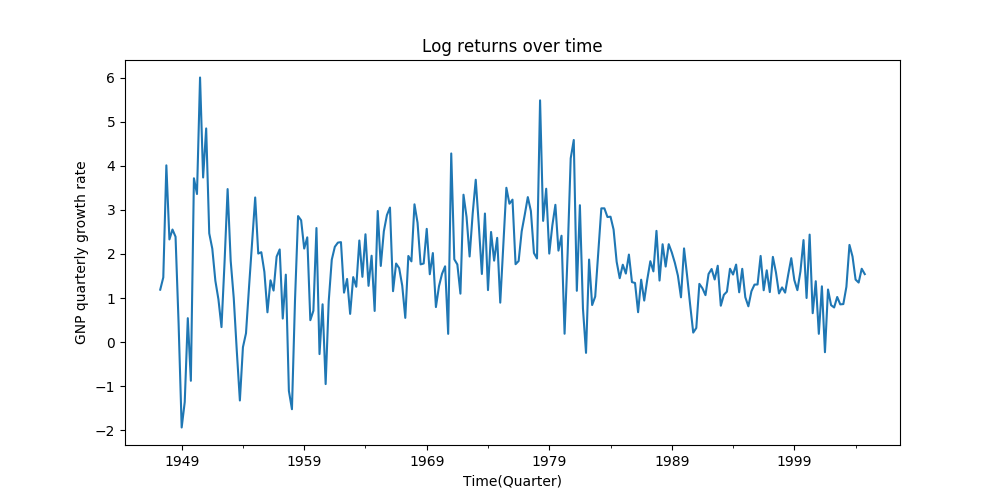
\includegraphics[width=1.2\textwidth]{/Users/tanvipotdar/Projects/Advanced-Numerical-Methods/modelling/log_returns.png}
    \caption{Log-returns for GNP training data}
\end{figure}
\item Plot of the Auto-correlation function of the training data
\begin{figure}[!htbp]
    \centering
    \vspace*{-1cm}
    \hspace*{-1cm}
    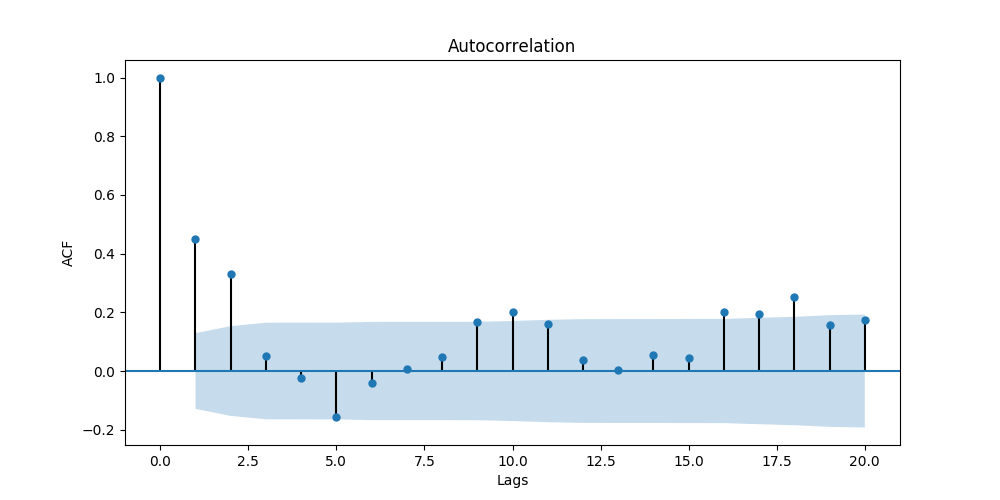
\includegraphics[width=1.2\textwidth]{/Users/tanvipotdar/Projects/Advanced-Numerical-Methods/modelling/acf}
    \caption{Autocorrelation plot for training data}
\end{figure}
\item Plot of the Partial auto-correlation function of the training data
\begin{figure}[!htbp]
    \centering
    \vspace*{-0.5cm}
    \hspace*{-1cm}
    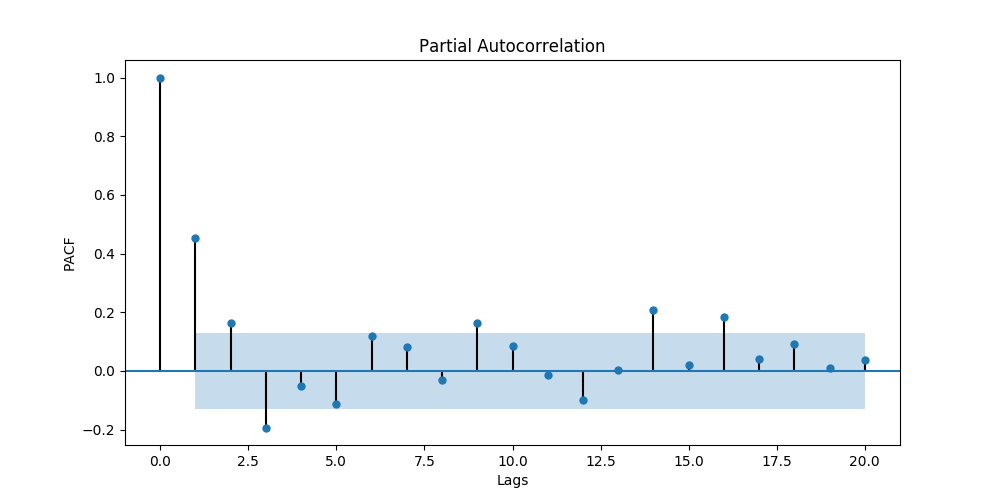
\includegraphics[width=1.2\textwidth]{/Users/tanvipotdar/Projects/Advanced-Numerical-Methods/modelling/pacf.png}
    \caption{Partial Autocorrelation plot for training data}
\end{figure}
\end{enumerate}
\item A multi-step ahead forecast is where we use time series observations up to a given period \textit{t} to generate a multi-step forecast \textit{k}(\textit{k}$>$1), where \textit{k} is the forecast horizon. Thus we use \textit{$y_t$} to generate a forecast for \textit{$y_{t+k}$}. A direct forecast models and estimates \textit{$y_{t+k}$} directly using a horizon specific model while an iterative forecast models and estimates \textit{$y_{t+1}$} first and iterates this forward until it reaches \textit{$y_{t+k}$}. A direct forecast is more robust to model mis-specification while an iterative forecast is better if the one step model is correctly specified. 
\end{enumerate}
\item Exponential Smoothing
\begin{enumerate}[label=(\alph*)]
\item Single exponential smoothing uses an exponential window function to smooth the time series data. While a simple moving average (MA) model assigns equal weights to past observations, SES uses exponential functions to assign decreasing weights to past observations with time. The smoothing factor $\alpha$ determines the rate of decay of old observations.  Setting the k-step ahead forecast:
\textit{$y_{t+k}$} = \textit{$s_t$}, we can define \textit{$s_t$} recursively as: \\
$s_0=y_0$
\newline 
\textit{$s_t$} = $\alpha$\textit{$y_t$} + $\alpha(1-\alpha)$\textit{$y_{t-1}$} + $\alpha(1-\alpha)^2$\textit{$y_{t-2}$} + ...
\newline
\textit{$s_t$} = $\alpha$\textit{$y_t$} + $(1-\alpha)$\textit{$s_{t-1}$}
\newline

\item Plot of in-sample SSE vs alpha:
\begin{figure}[!htbp]
    \centering
    \hspace*{-1cm}
    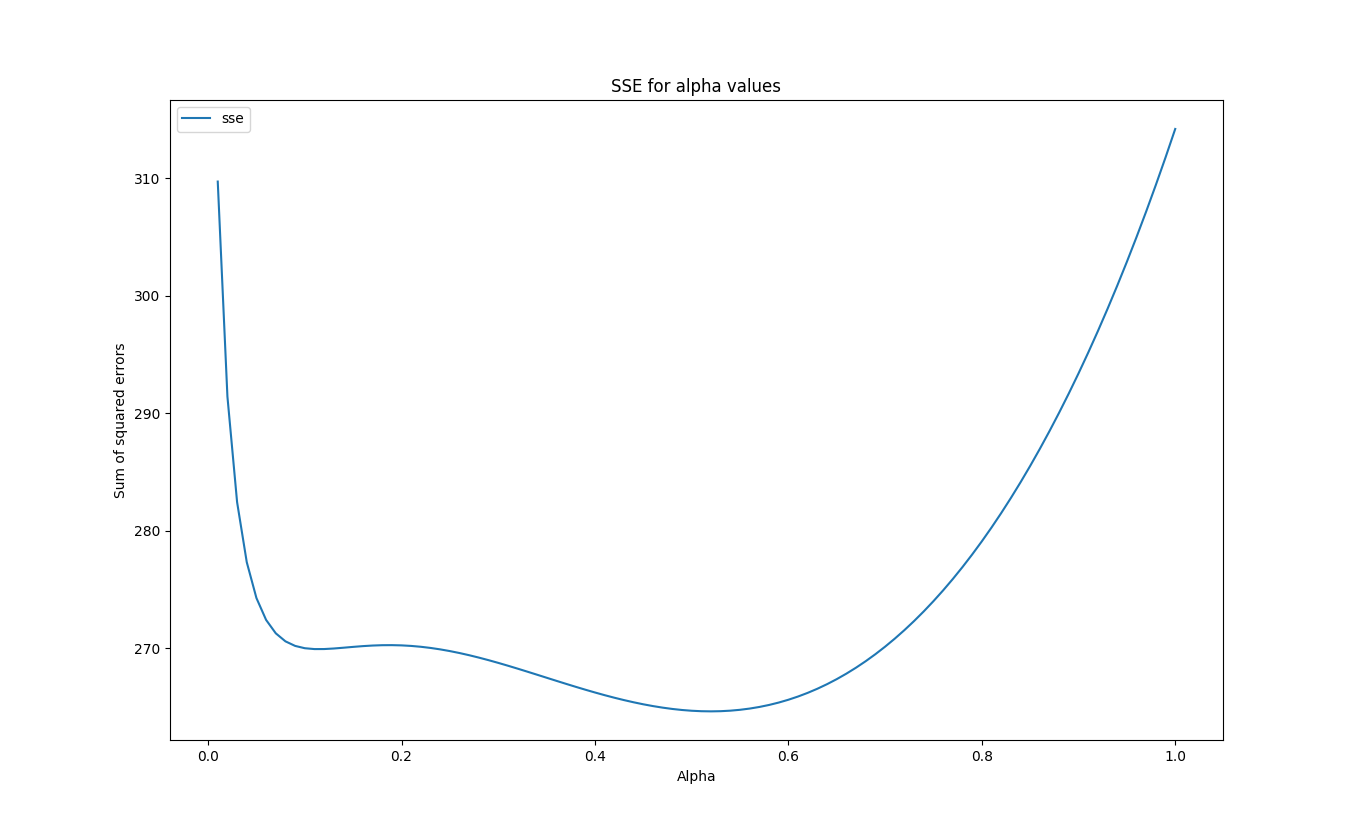
\includegraphics[width=1.2\textwidth]{/Users/tanvipotdar/Projects/Advanced-Numerical-Methods/modelling/alpha_vs_errors.png}
    \caption{In-sample SSE versus different values of the smoothing parameter $\alpha$}
\end{figure}
\item The optimal value of alpha that minimises the in-sample SSE is 0.52. Thus we can set $\alpha_{opt}=0.52$
\item Plot of in-sample model response along with the corresponding actual predictions:
\begin{figure}[!htbp]
    \centering
    \vspace*{-2cm}
    \hspace*{-1cm}
    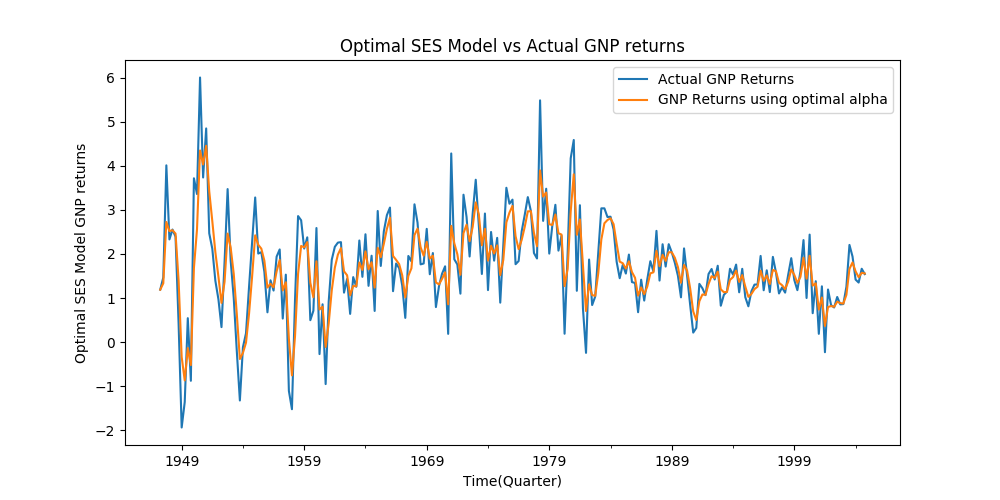
\includegraphics[width=1.2\textwidth]{/Users/tanvipotdar/Projects/Advanced-Numerical-Methods/modelling/optimal_ses_vs_actual_log_returns.png}
    \caption{In-sample optimal SES predictions vs actual observations for GNP log returns}
\end{figure}
\end{enumerate}
\item Auto-Regressive models
\begin{enumerate}[label=(\alph*)]
\item To find the optimal order, I experimented with the statsmodels package in Python, specifically the AR and ARMA models. Each of them gave me similar optimal orders. I chose to go with the ARMA model with q set to 0 for the MA part.  The optimal order of the Auto-Regressive model according to the ARMA model was 16. 
\item There are 17 coefficients for the AR(16) model.They are:
\begin{itemize}
    \item intercept = 1.68
    \item $\alpha_1$ = 0.38
    \item $\alpha_2$ = 0.23
    \item $\alpha_3$ = -0.12
    \item $\alpha_4$ = -0.0077
    \item $\alpha_5$ = -0.19
    \item $\alpha_6$ = 0.11
    \item $\alpha_7$ = 0.021
    \item $\alpha_8$ = -0.11
    \item $\alpha_9$ = 0.14
    \item $\alpha_{10}$ = 0.090
    \item $\alpha_{11}$ = 0.077
    \item $\alpha_{12}$ = -0.15
    \item $\alpha_{13}$ = -0.054
    \item $\alpha_{14}$ = 0.15
    \item $\alpha_{15}$ = -0.065
    \item $\alpha_{16}$ = 0.21
\end{itemize}
\end{enumerate}
\item Out-of-sample forecasting
\begin{enumerate}[label=(\alph*)]
\item Out-of-sample forecasting is used for model evaluation as a good fit on training data does not always translate into a good prediction on test data. 
\begin{itemize}
    \item Persistence - A persistence forecast corresponds to assuming that the underlying dynamics are generated by a random walk. Given a training data set $\{y_t\}$ and a horizon k, the prediction for $\hat{y}_{t+k}$ is:, the prediction for a data point $\hat{y}_{t+k}$ is $y_t$.  The forecasting scheme is given by the equation:  
      \[y_t \rightarrow \hat{y}_{t+k}\]\
 \item Climatology - The climatology forecast uses the distribution of the in-sample observations as a forecast for out-of-sample data. The unconditional average represents the expected value of the unconditional distribution of the training data. Given a training data set $\{y_t\}$ and a horizon k, the prediction for $\hat{y}_{t+k}$ is:
    \[\frac{1}{t}\sum_{i=1}^{t}{y_i}\rightarrow\hat{y}_{t+k} \]\
    Climatology forecasting does not give importance to the time ordering of the observations. Another idea is to take the mean of only the previous $\rho$ observations, where $\rho$ is estimated using cross validation.
    \item SES($\alpha_{opt}$) - Single exponential smoothing uses an exponential window function to smooth the time series data. While a simple moving average (MA) model assigns equal weights to past observations, SES uses exponential functions to assign decreasing weights to past observations with time. The smoothing factor $\alpha$ determines the rate of decay of old observations. Given a training data set $\{y_t\}$ and a horizon k, the prediction for $\hat{y}_{t+k}$ is:
 \begin{flalign*}
 s_t \rightarrow \hat{y}_{t+k} &\\
 s_t = \alpha_{opt}{y_t} + (1-\alpha_{opt})s_{t-1} &\\
 s_0 = y_0
\end{flalign*}
\item AR($p_{opt}$) - An AR($p$) model assumes a linear relationship between observations. The order $p$ refers to the number of lagged variables in the model. Forecast for out-of-sample points is the most recent observation. Given a training data set $\{y_t\}$ and a horizon k, the prediction for $\hat{y}_{t+k}$ is:
 \[y_t \rightarrow \hat{y}_{t+k}\]
  \[y_t  = \sum_{i=1}^{p}{\alpha_{i}y_{t-i}} + \epsilon_t, \epsilon\sim N(0,\sigma^2)\]\
  where $\alpha_i$ denotes AR model parameters and $y_t$ depends linearly on the previous $P$ values. 
\end{itemize}
\item Plot of out-of-sample optimal AR Model response along with the corresponding actual predictions and PDF of out-of-sample errors
\begin{figure}[!htbp]
    \centering
    \vspace*{-2cm}
    \hspace*{-1cm}
    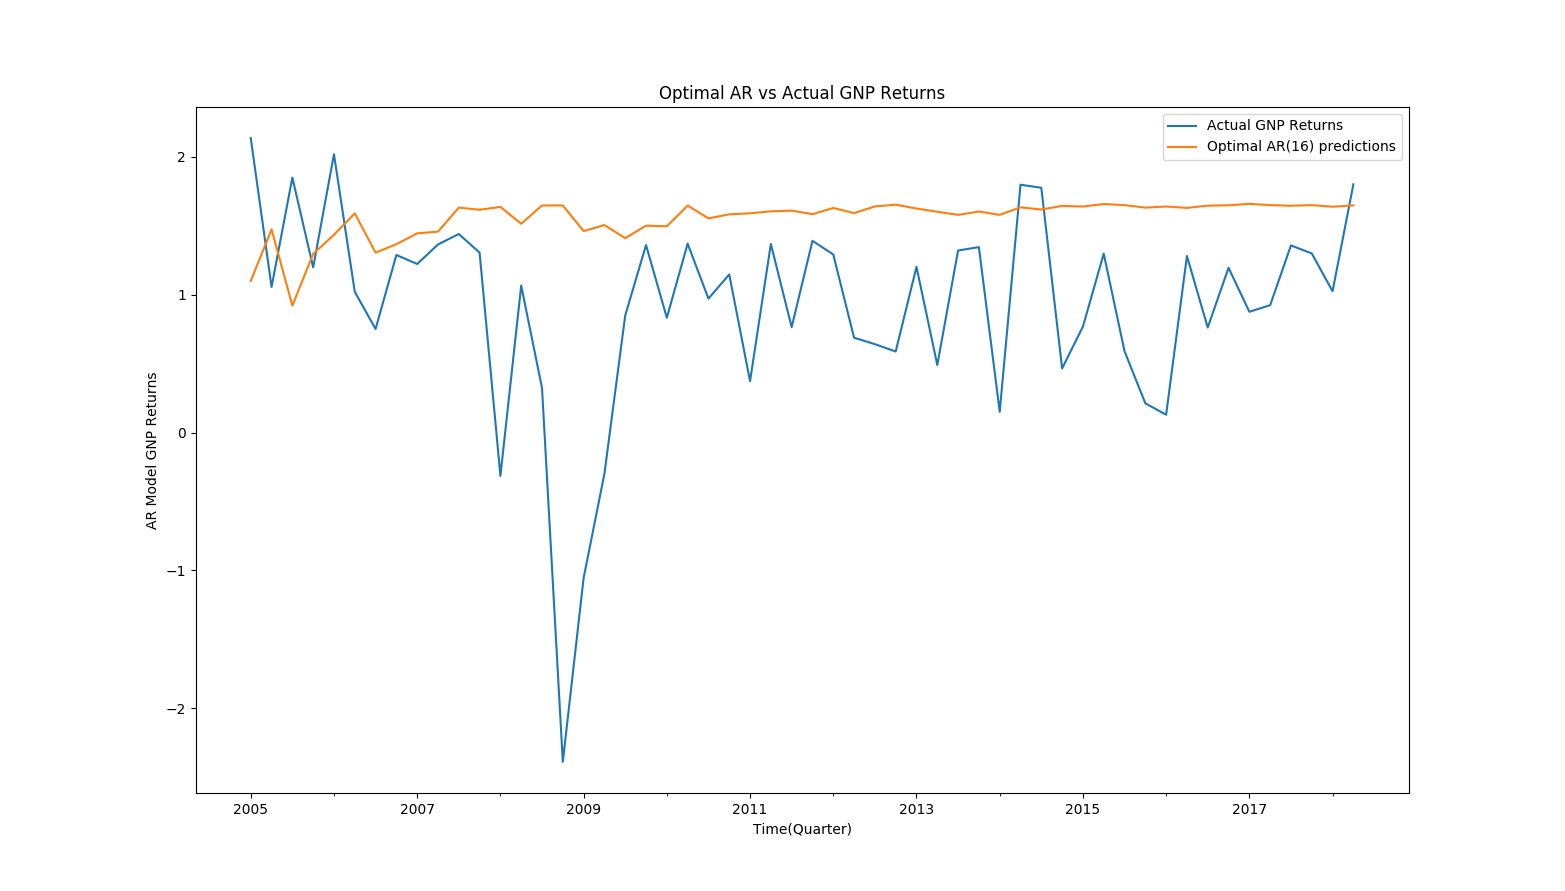
\includegraphics[width=1.2\columnwidth]{/Users/tanvipotdar/Projects/Advanced-Numerical-Methods/modelling/ar_vs_actual_gnp_returns}
    \caption{Out-of-sample optimal AR predictions vs testing data for GNP log returns}
\end{figure}
\begin{figure}[!htbp]
    \centering
    \vspace*{-1cm}
    \hspace*{-1cm}
    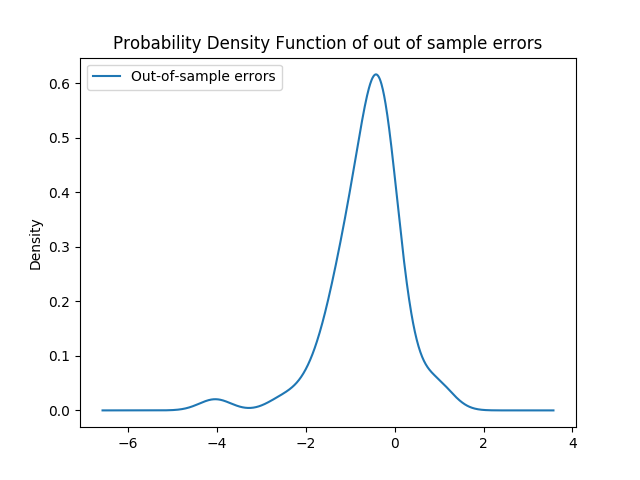
\includegraphics[width=1.2\columnwidth]{/Users/tanvipotdar/Projects/Advanced-Numerical-Methods/modelling/out_of_sample_errors_pdf}
    \caption{PDF of out of sample errors for the optimal AR model vs the testing data}
\end{figure}
\item Plot of out-of-sample root mean square error versus the forecast horizon for the four models - Persistence, Climatology, AR($p_{opt}$) and SES($\alpha_{opt}$)
\begin{figure}[!htbp]
    \centering
    \vspace*{-2cm}
    \hspace*{-1cm}
    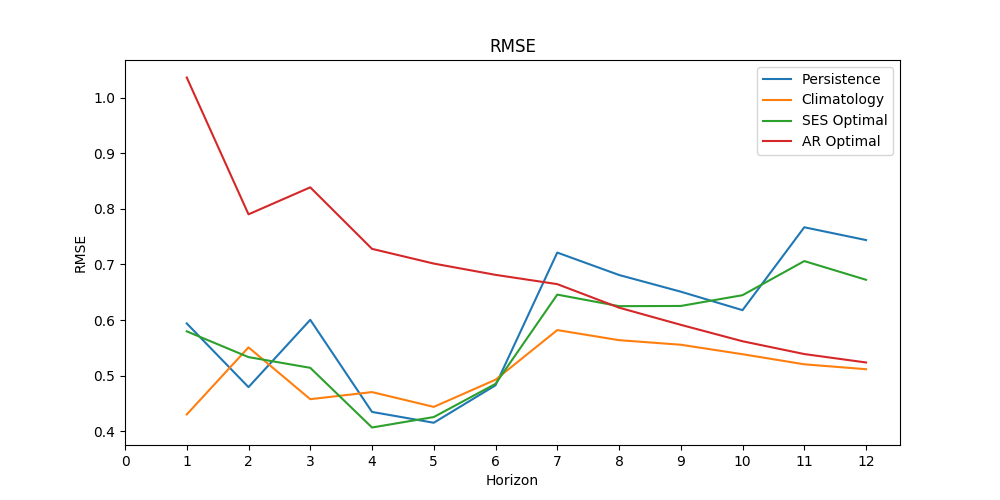
\includegraphics[width=1.2\columnwidth]{/Users/tanvipotdar/Projects/Advanced-Numerical-Methods/modelling/rmse_plot}
    \caption{Out-of-sample RMSE vs forecast horizon for four models}
\end{figure}
\item Plot of out-of-sample mean absolute error versus the forecast horizon for the four models - Persistence, Climatology, AR($p_{opt}$) and SES($\alpha_{opt}$)
\begin{figure}[!htbp]
  \centering
  \vspace*{-1cm}
  \hspace*{-1cm}
  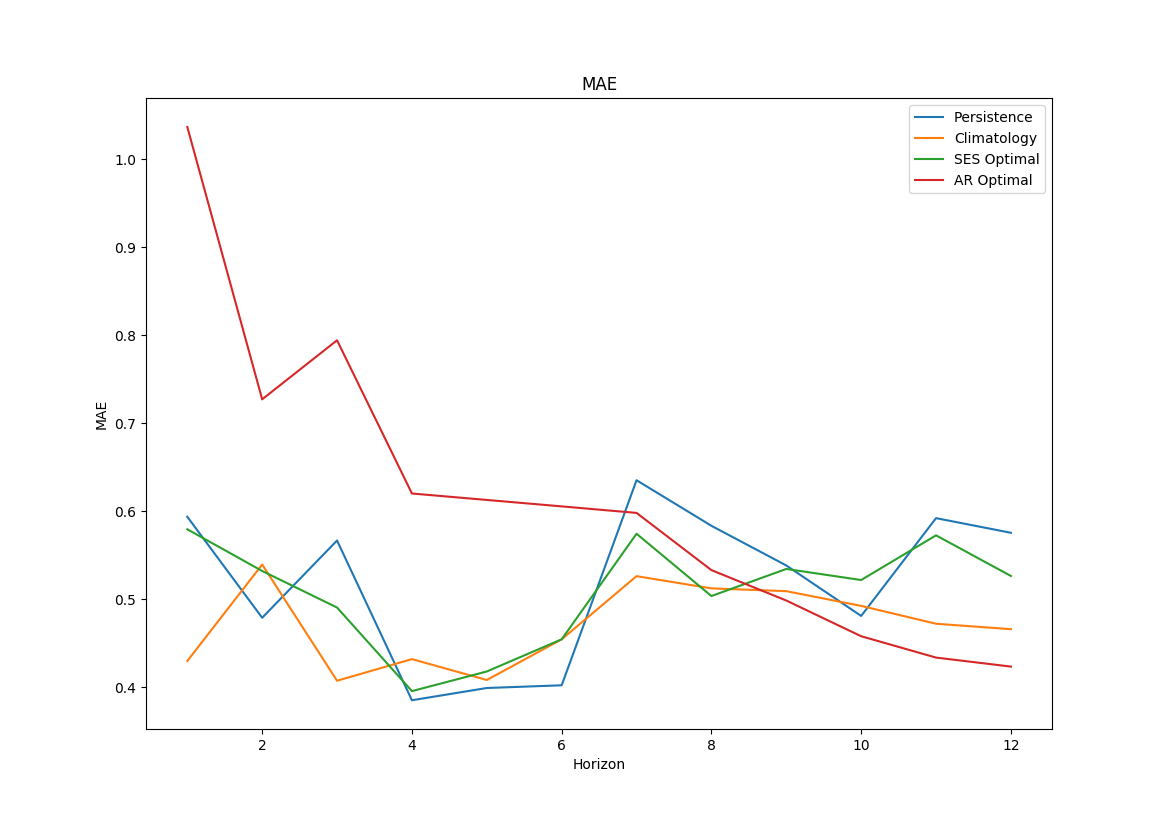
\includegraphics[width=1.2\columnwidth]{/Users/tanvipotdar/Projects/Advanced-Numerical-Methods/modelling/mae}
   \caption{Out-of-sample MAE vs forecast horizon for four models}
\end{figure}
\item Based on the mean absolute error and the root mean square error for the four models, the two best models are Climatology and the SES($\alpha_{opt}$). To generate an out-of-sample forecast using the Naive Composite, we take the average of the forecasts for each of these models. Figure 10 and 11 show the RMSE and MAE of all 5 models with the Naive Composite included.
\item The model with the most accurate out-of-sample forecast was the Climatology model, as can be seen in Fig 10 and 11. It has the lowest mean absolute error and root mean square error. This could be because it is the unconditional mean benchmark for the time-series. It assumes that the ordering of the data points does not provide additional information on future predictions which is true of the GNP data as a good or bad performance in one year does not necessarily mean the trend will continue. 
\begin{figure}[!htbp]
    \centering
    \hspace*{-1cm}
    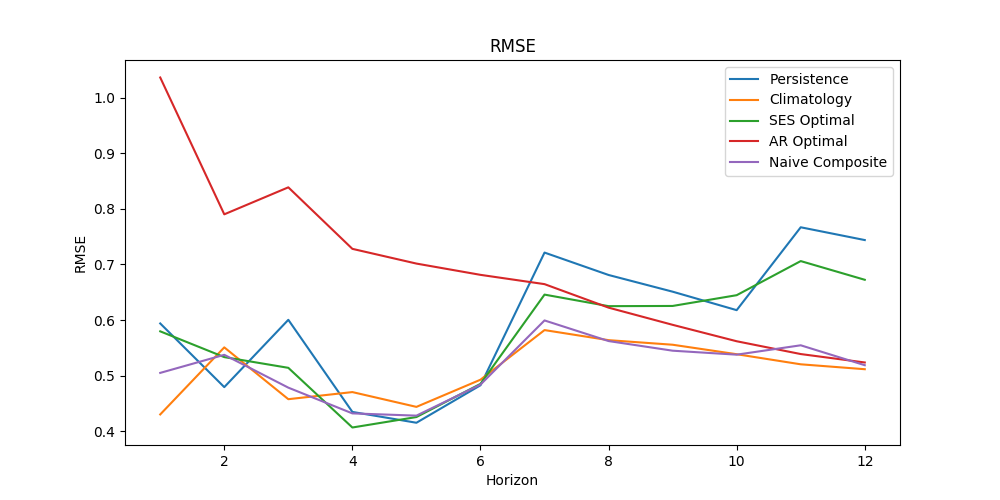
\includegraphics[width=1.2\columnwidth]{/Users/tanvipotdar/Projects/Advanced-Numerical-Methods/modelling/rmse_naive}
    \caption{Out-of-sample RMSE vs forecast horizon for five models including Naive Composite}
\end{figure}
\begin{figure}[!htbp]
  \centering
  \vspace*{-6.3cm}
  \hspace*{-1cm}
  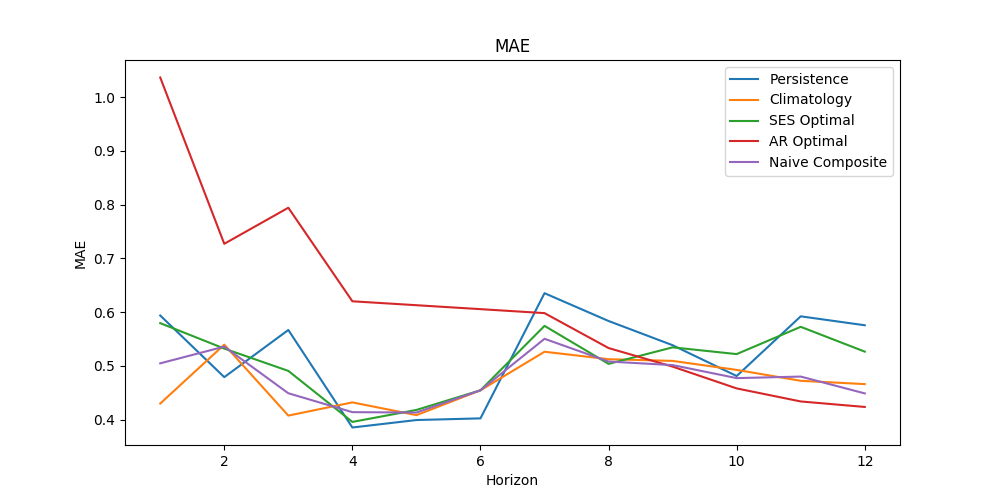
\includegraphics[width=1.2\columnwidth]{/Users/tanvipotdar/Projects/Advanced-Numerical-Methods/modelling/mae_naive}
   \caption{Out-of-sample MAE vs forecast horizon for five models including Naive Composite}
\end{figure}
\end{enumerate}
\end{enumerate}




\clearpage
\section{Appendix}
\begin{lstlisting}
import pandas as pd
import numpy as np
import matplotlib.pyplot as plt
from statsmodels.graphics.tsaplots import plot_acf, plot_pacf
from statsmodels.tsa.ar_model import AR
from statsmodels.tsa.arima_model import ARMA

#helper functions
 def f(x):            
	if x.year>2018:
		x = x.replace(year=x.year-100)
	return x

# 1.1
# set PATH accordingly
gnp_data = pd.read_csv(PATH, index_col='DATE')
log_returns = np.log(gnp_data.GNP/gnp_data.shift(1).GNP)*100
log_returns.dropna(inplace=True)
dates_index = pd.to_datetime(log_returns.index)
dates = map(f, dates_index)
log_returns.index = dates

training_data = log_returns[:231]
testing_data = log_returns[231:]


# plotting training data log returns
training_returns_plot, ax = plt.subplots(figsize=(10,5))
training_returns_plot = training_data.plot()
training_returns_plot.set(xlabel="Time(Quarter)", ylabel="GNP quarterly growth rate", title="Log returns over time")

# plotting training data acf
acf_plot, ax = plt.subplots(figsize=(10,5))
ax.set_xlabel('Lags')
ax.set_ylabel('ACF')
acf_plot = plot_acf(training_data, ax=ax, lags=20)


# plotting training data pacf
pacf_plot, ax = plt.subplots(figsize=(10,5))
ax.set_xlabel('Lags')
ax.set_ylabel('PACF')
pacf_plot = plot_pacf(training_data, ax=ax, lags=20)


# 1.2 Exponential Smoothing 
ses = training_data.to_frame('y')
alpha_values = np.arange(0.01, 1.01, 0.01)

for alpha in alpha_values:
	col_name = 's_{}'.format(alpha)
	#TODO: Check if this should be 1.0
	ses[col_name]=ses.y.tolist()[0]
	for i in range(1, len(ses)):
		ses[col_name][i] = ses[col_name][i-1]*(1-alpha) + alpha*ses.y[i]

errors = pd.DataFrame()
errors['alpha'] = alpha_values
error_vals = []
for alpha in alpha_values:    
	error_diff = (ses['s_{}'.format(alpha)].shift(1)-ses['y']).dropna()                  
	error_val = sum(error_diff**2)
	error_vals.append(error_val)

 errors['sse'] = error_vals
 errors.set_index('alpha', inplace=True)

# plot of alpha values versus in sample SSE
sse_plot, ax = plt.subplots(figsize=(10,5))
sse_plot = errors.plot(figsize=(10,5))
sse_plot.set(xlabel="Alpha", ylabel="Sum of squared errors (SSE)", title="SSE versus alpha")

# optimal value of alpha that minimises in sample SSE
optimal_alpha = errors.idxmin()

# plot of in-sample model response vs optimal alpha 
optimal_df = ses[['y', 's_0.52']]
optimal_df = optimal_df.rename(columns={'y':'Actual GNP Returns', 's_0.52':'GNP Returns using optimal alpha'})
optimal_plot = optimal_df.plot(figsize=(10,5))
optimal_plot.set(xlabel="Time(Quarter)", ylabel="Optimal SES Model GNP returns", title="Optimal SES Model vs Actual GNP returns")

# 1.3 Autoregressive models

min_aic = 20000000
min_order=0
for p in range(1,21):
	model = ARMA(training_data, order=(p,0))
	model_fit = model.fit()
	model_aic = model_fit.aic
	if model_aic < min_aic:
		min_aic = model_aic
		min_order = p

# Out of sample forecasting

persistence_forecast = []
climatology_forecast = []
ses_forecast = []
ar_forecast = []

avg_vals = [training_data[:-k].mean() if k>0 else training_data.mean() for k in range(12,-1,-1)]

ar_optimal = ARMA(training_data, order=(16,0))
ar_fit = ar_optimal.fit()
params = ar_fit.params
residuals = ar_fit.resid
p = ar_fit.k_ar
q = ar_fit.k_ma
k_exog = ar_fit.k_exog
k_trend = ar_fit.k_trend
for k in range(1,13):
	persistence_forecast.append(pd.Series(data=training_data[-k:].values, index=testing_data[:k].index))
	climatology_forecast.append(pd.Series(data = avg_vals[-k:], index=testing_data.index[:k]))
	ses_forecast.append(pd.Series(data=optimal_df['GNP Returns using optimal alpha'][-k:].values, index=testing_data[:k].index))
	ar_prediction = pd.Series(data=_arma_predict_out_of_sample(params, k, residuals, p, q, k_trend, k_exog, endog=training_data[1:], exog=None, start=len(training_data[1:])), index=testing_data[:k].index)
	ar_forecast.append(ar_prediction)

ar_prediction = pd.Series(data=_arma_predict_out_of_sample(params, len(testing_data), residuals, p, q, k_trend, k_exog, endog=training_data, exog=None, start=len(training_data)), index=testing_data.index)
preds=ar_prediction.to_frame('Optimal AR(16) predictions')
td =  testing_data.to_frame('Actual GNP Returns')
ar_vs_td = td.join(preds)

ar_vs_td_plot = ar_vs_td.plot(figsize=(10,5))
ar_vs_td_plot.set(xlabel="Time(Quarter)", ylabel="Optimal AR Model GNP Returns", title="Optimal AR vs Actual GNP Returns")

ar_vs_td['Out-of-sample errors'] = ar_vs_td['Actual GNP Returns'] - ar_vs_td['Optimal AR(16) predictions']
pdf_plot = ar_vs_td[['Out-of-sample errors']].plot.kde(figsize=(10,5))
pdf_plot.set(title="Probability Density Function of out of sample errors")

rmse_persistence_data = []
mae_per_data = []
for p in persistence_forecast:
	k = len(p)
	e = p - testing_data.head(k)
	rmse_persistence_data.append((e**2).mean()**.5)
	mae_per_data.append(e.abs().mean())
rmse_persistence = pd.Series(data=rmse_persistence_data, index=range(1,13)).to_frame('Persistence')
mae_persistence = pd.Series(data=mae_per_data, index=range(1,13)).to_frame('Persistence')

rmse_climatology_data = []
mae_clim_data = []
for p in climatology_forecast:
	k = len(p)
	e = p - testing_data.head(k)
	rmse_climatology_data.append((e**2).mean()**.5)
	mae_clim_data.append(e.abs().mean())
rmse_climatology = pd.Series(data=rmse_climatology_data, index=range(1,13)).to_frame('Climatology')
mae_climatology = pd.Series(data=mae_clim_data, index=range(1,13)).to_frame('Climatology')

rmse_ses_data = []
ses_mae_data = []
for p in ses_forecast:
	k = len(p)
	e = p - testing_data.head(k)
	rmse_ses_data.append((e**2).mean()**.5)
	ses_mae_data.append(e.abs().mean())
rmse_ses = pd.Series(data=rmse_ses_data, index=range(1,13)).to_frame('SES Optimal')
mae_ses = pd.Series(data=ses_mae_data, index=range(1,13)).to_frame('SES Optimal')


rmse_ar_data = []
mae_ar_data = []
for p in ar_forecast:
	k = len(p)
	e = p - testing_data.head(k)
	rmse_ar_data.append((e**2).mean()**.5)
	mae_ar_data.append(e.abs().mean())
rmse_ar = pd.Series(data=rmse_ar_data, index=range(1,13)).to_frame('AR Optimal')
mae_ar = pd.Series(data=mae_ar_data, index=range(1,13)).to_frame('AR Optimal')


rmse_df = rmse_persistence.join(rmse_climatology).join(rmse_ses).join(rmse_ar)
rmse_plot = rmse_df.plot(figsize=(10,5))
rmse_plot.set(xlabel="Horizon", ylabel="RMSE", title="RMSE")


mae_df = mae_persistence.join(mae_climatology).join(mae_ses).join(mae_ar)
mae_plot = mae_df.plot(figsize=(10,5))
mae_plot.set(xlabel="Horizon", ylabel="MAE", title="MAE")

# naive composite forecast scheme
naive_composite = [(climatology_forecast[i]+ses_forecast[i])/2 for i,x in enumerate(climatology_forecast)]

rmse_naive_data = []
mae_naive_data = []
for p in naive_composite:
	k = len(p)
	e = p - testing_data.head(k)
	rmse_naive_data.append((e**2).mean()**.5)
	mae_naive_data.append(e.abs().mean())
rmse_naive = pd.Series(data=rmse_naive_data, index=range(1,13)).to_frame('Naive Composite')
mae_naive = pd.Series(data=mae_naive_data, index=range(1,13)).to_frame('Naive Composite') 

rmse_df['Naive Composite'] = rmse_naive['Naive Composite']
mae_df['Naive Composite'] = mae_naive['Naive Composite']

rmse_naive_plot = rmse_df.plot(figsize=(10,5))
rmse_naive_plot.set(xlabel="Horizon", ylabel="RMSE", title="RMSE")
mae_naive_plot = mae_df.plot(figsize=(10,5))
mae_naive_plot.set(xlabel="Horizon", ylabel="MAE", title="MAE")

\end{lstlisting}
\end{document}
